\maketitle

\
{\em Coding theory} is a branch of mathematics and computer science that deals with the properties of {\em codes} and their respective fitness for specific applications. One of the key areas of research in coding theory is the study of bounds on the performance of codes: two of the most important bounds in this area are the {\em sphere-packing bound} and the {\em Delsarte bound}. In this brief article, we will take a closer look at these bounds, exploring their key concepts and applications in modern coding theory, in order to show how they can be used to optimize the performance of a code.


\section{Introduction}
Suppose we're trying to build a remote with 16 keys for a DVD player. The most natural option would be to transmit 4-bit sequences, since there are $2^4=16$ possible sequences (or {\em words}) that can be arranged with 4 bits.

However, a problem arises as soon as the situation gets more realistic. If the transmission is not reliable, there is a probability for each bit in the transmission to be received incorrectly; this will lead to a lot of wrong inputs and is thus a flaw of the device.

We could try reducing the error rate by tripling each of the four transmitted bits, so instead of tarnsmitting {\em abcd} we would transmit {\em aaabbbcccddd}, but this leads to another problem: we're using 12 bits! This will exhaust the battery of our remote control much faster.

\begin{definition}[Hamming distance]
Given two code words $\textbf{w}, \textbf{w}' \in \{0,1\}^n$, the \emph{Hamming distance} between $\textbf{w}$ and $\textbf{w}'$ is the number of bits in which $\textbf{w}$ differs from $\textbf{w}'$:

\begin{equation}
    d_H(\textbf{w}, \textbf{w}') := |\{j \in \{1, 2, \ldots, n\} : w_j \neq w_j'\}|.
\end{equation}
\end{definition}
In other words, the Hamming distance is the number of errors (bit flips) that need to occur for \textbf{w} to become \textbf{w'}.

\begin{example}
If $n = 3$, we can form $2^3=8$ unique code words, with the following distances from each other:

\begin{table}[!ht]
    \centering
    \begin{tabular}{|c|c|c|c|c|c|c|c|c|}
    \hline
        \textbf{$d_H$} & \textbf{101} & \textbf{111} & \textbf{011} & \textbf{001} & \textbf{000} & \textbf{010} & \textbf{110} & \textbf{100} \\ \hline
        \textbf{101} & 0 & 1 & 2 & 1 & 2 & 3 & 2 & 1 \\ \hline
        \textbf{111} & 1 & 0 & 1 & 2 & 3 & 2 & 1 & 2 \\ \hline
        \textbf{011} & 2 & 1 & 0 & 1 & 2 & 1 & 2 & 3 \\ \hline
        \textbf{001} & 1 & 2 & 1 & 0 & 1 & 2 & 3 & 2 \\ \hline
        \textbf{000} & 2 & 3 & 2 & 1 & 0 & 1 & 2 & 1 \\ \hline
        \textbf{010} & 3 & 2 & 1 & 2 & 1 & 0 & 1 & 2 \\ \hline
        \textbf{110} & 2 & 1 & 2 & 3 & 2 & 1 & 0 & 1 \\ \hline
        \textbf{100} & 1 & 2 & 3 & 2 & 1 & 2 & 1 & 0 \\ \hline
    \end{tabular}
    \caption{Hamming distances for all possible code words with $n=3$}
\end{table}

Another way to visualize the Hamming distance is by putting each possible code word in the vertices of a (hyper)cube. Of course, for $n=2$ the cube becomes a square. If every word is placed such that it has only one bit of difference with respect to each of its neighbors, then the Hamming distance between two words will be the number of edges we need to traverse in order to get from one word to the other.

\begin{figure}
    \centering
    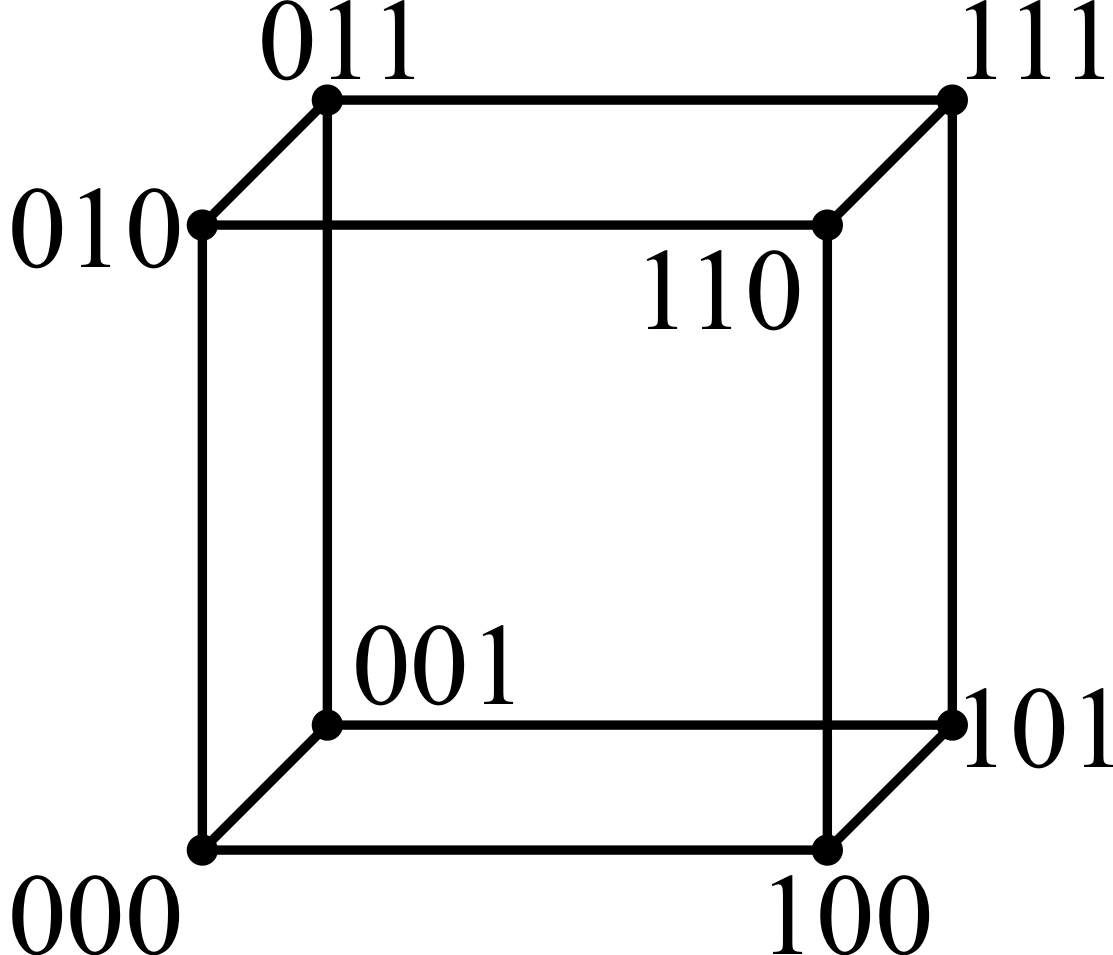
\includegraphics[width=0.25\textwidth]{hamming-cube.png}
\caption{Hamming cube for $n=3$}
\end{figure}

\end{example}

\begin{definition}[weight of a code-word]
Suppose $\textbf{w}$ is a code-word such that $\textbf{w} \in \{0,1\}^n$. The \emph{weight} of $\textbf{w}$ is the number of 1's in $\textbf{w}$:

\begin{equation}
    |\textbf{w}| := |\{j \in \{1, 2, \ldots, n\} : w_j = 1\}|.
\end{equation}

\end{definition}
\begin{example}
Suppose $n=5$.
\begin{equation*}
    |(1, 0, 0, 1, 1)| = 3 \quad\quad |(1, 0, 0, 0, 0)| = 1 \quad\quad |(0, 0, 1, 1, 1)| = 4
\end{equation*}
\end{example}

\begin{definition}[sum modulo 2 (bit-wise xor)]
Given two words $\textbf{w}, \textbf{w}' \in \{0,1\}^n$, we can define the following operation:
\begin{equation}
    \textbf{w} \oplus \textbf{w}' = ((w_1 + w_1')\text{mod}2, (w_2 + w_2')\text{mod}2, \ldots, (w_n + w_n')\text{mod}2) \in \{0,1\}^n
\end{equation}
\end{definition}
The \emph{sum modulo 2} operation returns a vector of size $n$ where each component  $z_j$ has value:
\begin{itemize}
    \item 0 if $w_j = w_j'$;
    \item 1 if $w_j \neq w_j'$
\end{itemize}

\begin{example}
Suppose $n=6, \textbf{w} = (1, 1, 0, 0, 1, 0), \textbf{w}' = (0, 1, 1, 0, 0, 1)$.
\begin{equation*}
\begin{array}{l}
(1, 1, 0, 0, 1, 0) \,+ \\
(0, 1, 1, 0, 0, 1) = \\  \hline
(1, 2, 1, 0, 1, 1)
\end{array}
\quad\rightarrow\quad
\begin{array}{l}
(1, 2, 1, 0, 1, 1)\text{mod} 2 = \\ \hline
(1, 0, 1, 0, 1, 1) = \textbf{w} \oplus \textbf{w}'
\end{array}.
\end{equation*}
\end{example}

At this point, it's clear how this identity holds true:
\begin{equation}
    d_H(\textbf{w}, \textbf{w}') = |\textbf{w} \oplus \textbf{w}'|
\end{equation}
Which means: the weight of the result obtained from the bit-wise xor operation is the Hamming distance between the two code-words.

\begin{proposition}
    The number of words with Hamming distance exactly $i$ from a given word $\mathbf{w}$ is ${ n \choose i }$:

    \begin{equation}
        |\{ \mathbf{w} \in \{0,1\}^n : d_H(\mathbf{w},\mathbf{w}') = i\}| = {n \choose i}\quad \forall \mathbf{w'} \in \{0,1\}^n.
    \end{equation}
\end{proposition}
\begin{example}
    Suppose we want to count the words which have distance $i=2$ from the word $001$ ($n=3$).
    
    \begin{equation*}
        \begin{aligned}
            \mathbf{w} = 001 \\
            n = 3 \\
            i = 2 
        \end{aligned}
        \quad
        \left.\begin{aligned}
            111\\
            101\\
            110
        \end{aligned}
        \right\} 3
        \quad\quad
        \begin{aligned}
            \mathbf{w} = 10010 \\
            n = 5 \\
            i = 4
        \end{aligned}
        \quad
        \left.\begin{aligned}
            01100\\
            11101\\
            00101\\
            01011\\
            01101
        \end{aligned}
        \right\} 5
    \end{equation*}

    \begin{equation*}
        {3 \choose 2} = \frac{3!}{2!(3-2)!}=\frac{3!}{2!}=3
        \quad\quad
        {5 \choose 4} = \frac{5!}{4!(5-4)!}=\frac{5!}{4!}=5
    \end{equation*}

\end{example}

\begin{definition}[distance of a code]
In coding theory, any subset $\mathcal{C} \subseteq \{0,1\}^n$ is called a \emph{code}.

A code $\mathcal{C}$ has \emph{distance} $d$ if:

\begin{equation}
    d_H(\textbf{w}, \textbf{w}') \geq d \quad \forall \;\textbf{w}, \textbf{w}' \in \mathcal{C}.
\end{equation}

Lastly, for $n, d \geq 0$, let $A(n,d)$ denote the maximum cardinality of a code $\mathcal{C} \subseteq \{0,1\}^n$ with distance $d$.
\end{definition}

\begin{example}
For $n=7$, a valid code of distance $d=3$ could be the set:

\begin{equation*}
\label{sample-code}
\mathcal{C} =
\left.
\begin{cases}
& 0000000, 0001011, 0010101, 0011110, \;\;\;\\
& 0100110, 0101101, 0110011, 0111000, \\
& 1000111, 1001100, 1010010, 1011001, \\
& 1100001, 1101010, 1110100, 1111111 
\end{cases}\right\}.
\end{equation*}

Notice how, in this code, every two distinct words have an Hamming distance of at least $3$.
\end{example}

\begin{proposition}
A code $\mathcal{C}$ can correct at most $r$ errors if and only if it has distance $d \geq 2r+1$.
\end{proposition}
\begin{example}
    Suppose $\mathcal{C}$ contains two distinct words $\textbf{w}', \textbf{w}''$ that differ in at most $2r$ bits. For example, with $n=7$ and $r=1$, suppose we receive $\hat{\textbf{w}}$, obtained by flipping $r=1$ bits in one of them:
\begin{equation*}
\textbf{w}' = 0000011 \quad \textbf{w}'' =0000101 \quad \hat{\textbf{w}} = 0000001
\end{equation*}
At this point, it's impossible to know whether the originally transmitted word was $\textbf{w}'$ or $\textbf{w}''$. This test can be repeated by choosing any code with distance $d=2r$ and flipping $r$ of them.

On the other hand, if $\mathcal{C}$ had a distance of $2r+1$, we would be sure it could correct up to $r$ errors:

\begin{equation*}
\textbf{w}' = 0000011 \quad \textbf{w}'' =0010101 \quad \hat{\textbf{w}} = 0000001
\end{equation*}

In this case, we can be sure that $\textbf{w}''$ was transmitted.
\end{example}

In most cases, the number $n$ of bits we can transmit and the amount of errors $r$ to be corrected are given; one of the main problems of coding theory (and the main topic of this document) is finding $A(n,d)$, the maximum possible size of a code $\mathcal{C} \subseteq \{0,1\}^n$ with distance $d$.

\section{Simple cases}
\subsection*{$d=1$}
First of all, any code needs to have distance 1 by definition: otherwise, we would not be able to distinguish between code words. That said, for all $n$, we always have $A(n,1) = 2^n$, which is the number of possible codewords of $n$ bits.

\subsection*{$d=2$}
To get $A(n,2)$ we start by considering a particular code.
\begin{lemma}
    The code $\mathcal{C}$, composed by all $n$-bit codewords of even weight, has distance 2.
\end{lemma}
\subsubsection*{Proof}
We need to prove two things:
\begin{enumerate}
    \item $\exists (\mathbf{w},\mathbf{w}') : d_H(\mathbf{w},\mathbf{w}')=2\quad\forall\; \mathbf{w},\mathbf{w}' \in \mathcal{C}$
    \item $\nexists (\mathbf{w},\mathbf{w}') : d_H(\mathbf{w},\mathbf{w}')=1\quad\forall\; \mathbf{w},\mathbf{w}' \in \mathcal{C}$
\end{enumerate}

To prove point 1, we can just take any word $\mathbf{w}\in \mathcal{C}:|\mathbf{w}|\geq 2$. Then, consider the word $\mathbf{w}'$, obtained by replacing two of the 1's in the word with two 0's.
$\mathbf{w}'$ has even weight, so we have $\mathbf{w}' \in \mathcal{C}$.

As for point 2, we use a proof by contradiction to show how it's impossible for two words in the code to have distance 1.

Let $\mathbf{w},\mathbf{w}' \in \mathcal{C}$ and suppose $d_H(\mathbf{w},\mathbf{w}')=1$. If $\mathbf{w}$ and $\mathbf{w}'$ have Hamming distance 1, they differ in only 1 bit.
This means that if $\mathbf{w}$ has even weight, $\mathbf{w}'$ has to have odd weight, and viceversa. This is a contradiction to the hypothesis of all words in $\mathcal{C}$ having even weight, so $\mathbf{w}$ and $\mathbf{w}'$ cannot have Hamming distance 1.

Finally, let's find an upper bound for this code.
\begin{lemma}
    Fixed $n$, if $ \mathcal{C} \subseteq \{0,1\}^n : |w| \text{ is even }\forall\; \mathbf{w}\in \mathcal{C}$, then $|\mathcal{C}| \geq 2^{n-1}$.%TODO: should be equal?
\end{lemma}
\subsubsection*{Proof}
We know that the total number of words in a $n$-bit code is $2^n$. We start with a code made up of $(n-1)$-bit words, and consider the code $\mathcal{C} \subseteq \{0,1\}^n$ obtained by applying the following transformation to each word of the code:
\begin{itemize}
    \item if the word has an even weight, add a $0$;
    \item if the word has an odd weight, add a $1$.
\end{itemize}

We obtained a code $\mathcal{C}$ which is composed by all the codewords with even weight. Furthermore, $|\mathcal{C}| \geq 2^{n-1}$, which was the number of elements in the starting code. %TODO: should be equal?

This is proof that, for any value of $n$, $A(n,2) = 2^{n-1}$.

\subsection*{$d\geq 3$}
The previous values of $d$ didn't allow for space to correct any errors.

%TODO: show that you need 2r+1 distance to correct r errors.
Unfortunately, for $d \geq 3$, things start to get complicated.

\subsection{The sphere-packing bound}

For any $n$ and $d$, we can use a \emph{volume argument} to obtain a simple upper bound on $A(n, d)$.

Imagine a box filled with balls. If you wanted to guess how many balls can fit inside it, you could conclude that the number of balls is bounded above by the volume of the container divided by the volume of a single ball.

Let's assume that $d = 2r+1$ is odd and fix any code $\mathcal{C}$ of distance $d$. Now, the set $\{0,1\}^n$ represents the box, containing $|\mathcal{C}|$ Hamming balls. Each ball is defined as the set of all words in $\{0,1\}^n$ with a distance $r$ from a certain word $w \in \mathcal{C}$.
\begin{equation}
    B(\mathbf{w}, r) := \{\mathbf{w}' \in \{0,1\}^n : d_H(\mathbf{w}, \mathbf{w}') \leq r\}, \mathbf{w} \in \mathcal{C}.
\end{equation}

\begin{figure}[ht!]
    \label{sphere-vis}
    \centering
    \fbox{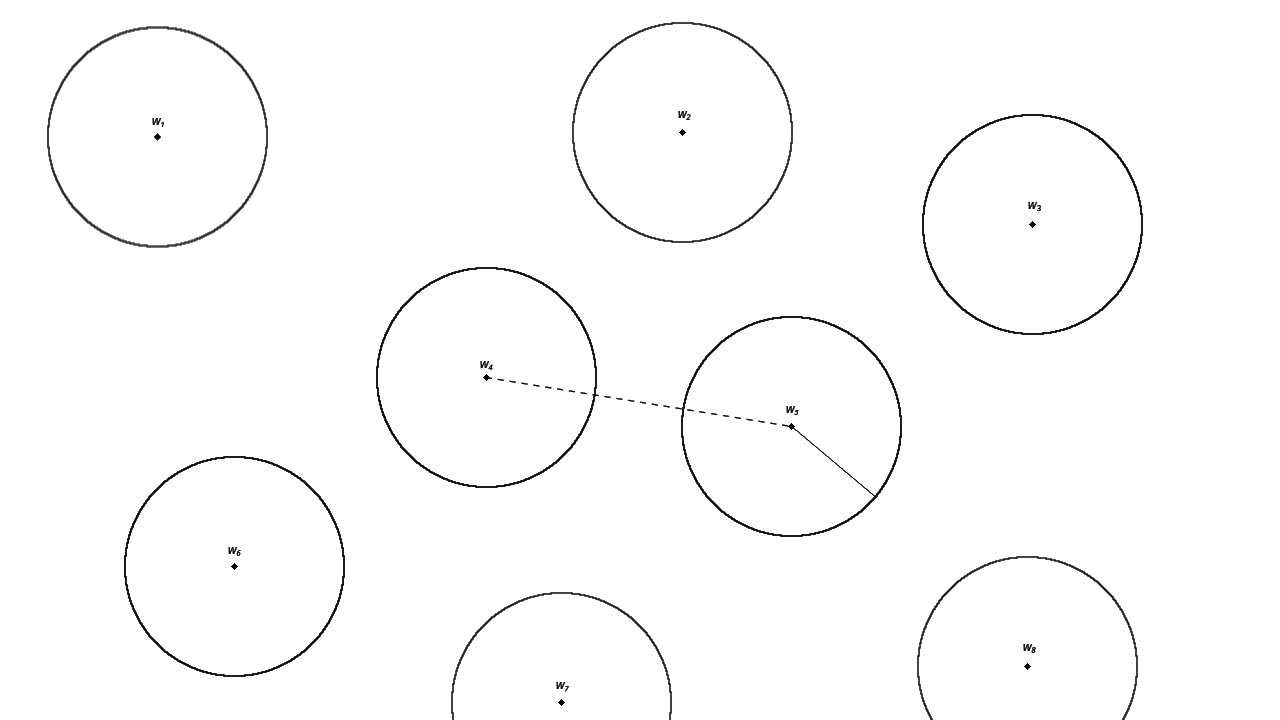
\includegraphics[width=\textwidth]{sphere-packing.png}}
\caption{A visualization of the sphere-packing bound.}
\end{figure}

So we have $|\mathcal{C}|$ balls of radius $r$ and distance at least $2r+1$ from one another. This means the balls are disjoint, they're not overlapped. The total number of balls (words in $\mathcal{C}$) cannot be larger than the total number of words in $\{0,1\}^n$  divided by the number of words in a single ball.

The number of words at Hamming distance exactly $i$ from any word $w$ is ${n \choose i}$, which implies:

\begin{equation*}
    |B(\mathbf{w}, r)| = 1 + {n \choose 1} + {n \choose 2} + \dots + {n \choose r} = \sum_{i=0}^{r} {n \choose i},
\end{equation*}
where each iteration of the sum adds the amount of elements of weight $i$.

Finally, as we said before, the total number of elements in $\{0,1\}^n$ is $2^n$. So, we get the following upper bound:

\begin{lemma}[sphere-packing bound]
    For all n and r,

    \begin{equation}
        A(n, 2r+1) \leq \floor*{\frac{2^n}{\sum\limits_{i=0}^{r}{n \choose i}}}.
    \end{equation}
\end{lemma}

\begin{example}
    For $n=7$ and $d=3$, we have $r=1$ so:
    \begin{equation*}
        A(7,3) \leq \floor*{\frac{2^7}{\sum\limits_{i=0}^{1}{7 \choose i}}} = \floor*{\frac{128}{{7 \choose 0} + {7 \choose 1}}} = \floor*{\frac{128}{1 + 7}} = 16.
    \end{equation*}
\end{example}

\begin{example}
    For $n=17$ and $d=3$:
    \begin{equation*}
        A(17,3) \leq \floor*{\frac{2^{17}}{\sum\limits_{i=0}^{1}{17 \choose i}}} = \floor*{\frac{131072}{{17 \choose 0} + {17 \choose 1}}} = \floor*{\frac{131072}{1 + 17}} = 7281.
    \end{equation*}
\end{example}

\section{The Delsarte bound}
\begin{theorem}[Delsarte bound]
    For integers $n$, $i$, $t$ with $0 \leq i$, $t \leq n$, let us put

    \begin{equation}
        K_t(n,i) = \sum_{j=0}^{min(i,t)}(-1)^j{i \choose j}{n - i \choose t - j}.
    \end{equation}
    where $K_t$ is the \emph{Krawtchouk polynomial} of degree $t$.

    Then, for every $n$ and $d$, $A(n,d)$ is bounded above by the optimum value of the following linear program in variables $x_0, x_1, \ldots, x_n$:

    \begin{equation}
        \begin{array}{lll}
            \text{Maximize}   & x_0 + x_1 + \ldots + x_n                       &                  \\
            \text{subject to} & x_0 = 1                                        &                  \\
                              & x_i = 0,                                       & i=1,2,\ldots,d-1 \\
                              & \sum\limits_{i=0}^{n}K_t(n,i) \cdot x_i \geq 0, & t=1,2,\ldots,n   \\
                              & x_0, x_1, \ldots, x_n \geq 0                   &                  \\
        \end{array}
    \end{equation}
\end{theorem}

\subsection{Making sense of these constraints}
For each code $\mathcal{C} \subseteq \{0,1\}^n$ we associate $\mathbf{\tilde{x}}=(\tilde{x}_1, \tilde{x}_2, \ldots, \tilde{x}_n)$ such that each $\tilde{x}_i$ is a nonnegative real number and $\tilde{x}_1+\tilde{x}_2+\ldots+\tilde{x}_n=|\mathcal{C}|$.
We need to prove that, if $\mathcal{C}$ has distance $d$, then $\mathbf{\tilde{x}}$ is a feasible solution for Delsarte's linear program.
The optimal solution of that linear program (the maximum) is greater or equal to the size of any existing code $\mathcal{C}$ with distance $d$. % TODO: rivedere questa cosa???
Given $\mathcal{C} \subseteq \{0,1\}^n$, we define each $\tilde{x}_i$ as the number of words in $\mathcal{C}$ which have distance $i$, divided by the total number of words in $\mathcal{C}$:
\begin{equation}
    \label{xtildei}
    \tilde{x}_i = \frac{1}{|\mathcal{C}|} | \{ (\mathbf{w}, \mathbf{w}')\in\mathcal{C}^2:d_H(\mathbf{w}, \mathbf{w}')=i\}|, \quad i=0,1, \ldots,n.
\end{equation}
We compute $\tilde{x}_i$ by looking at $\mathcal{C}^2$, so we're counting couples of words with a certain distance $i$. A single couple of words cannot have two different distances, so each couple contributes to one and only one of the $\tilde{x}_i$ variables. For this reason, we have $\tilde{x}_1+\tilde{x}_2+\ldots+\tilde{x}_n=|\mathcal{C}|$.
Furthermore, since every word only has distance 0 from itself, $\tilde{x}_0$ will always be equal to $\frac{|\mathcal{C}|}{|\mathcal{C}|}=1$.
If our code $\mathcal{C}$ has distance $d$, then every word in it has distance greater or equal than $d$ from other words. That means $\tilde{x}_1, \tilde{x}_2, \ldots, \tilde{x}_{d-1}=0$.
\begin{example}
    Let's try computing $\mathbf{\tilde{x}}$ for a simple code.
    \begin{equation*}
        \mathcal{C} \; = \{000, 001, 101, 111\} \quad\quad |\mathcal{C}|=4 \quad\quad n=3
    \end{equation*}
    \begin{equation*}
        \begin{array}{l}
            \tilde{x}_0 = \frac{1}{4}|\{(000,000), (001, 001), (101, 101), (111, 111)\}|=\frac{4}{4}=1 \\\\
            \tilde{x}_1 = \frac{1}{4}|\{(000,001), (001,000), (001,101), (101, 001), (101, 111), (111, 101)\}|=\frac{6}{4}=\frac{3}{2}\\\\
            \tilde{x}_2 = \frac{1}{4}|\{(001,111), (111, 001), (000,101), (101, 000)\}|=\frac{4}{4}=1\\\\
            \tilde{x}_3 = \frac{1}{4}|\{(000,111), (111, 000)\}|=\frac{2}{4}=\frac{1}{2}\\\\
            \tilde{x}_0 + \tilde{x}_1 + \tilde{x}_2 + \tilde{x}_3 = 1 + \frac{3}{2} + 1 + \frac{1}{2} = 4 = |\mathcal{C}|
        \end{array}
    \end{equation*}
\end{example}
\subsection{The final constraint}
Let $\mathcal{C} \subseteq \{0,1\}^n$ be an arbitrary set, and let $\tilde{x}_i$ be defined as above (\ref{xtildei}) for $i=0,1,\ldots,n$ and $t=1,2,\ldots,n$.
Then,
\begin{equation*}
    \sum_{i=0}^{n}K_t(n,i) \tilde{x}_i \geq 0.
\end{equation*}
To prove this, let $I \subseteq \{1,2,\ldots n\}$ be a set of indices and let's define the Hamming distance $d_H^I(\mathbf{w}, \mathbf{w}')$ as the largest number of indices $i \in I$ with $w_i \neq w_i'$:
\begin{equation}
    d_H^I(\mathbf{w}, \mathbf{w}') = |\{i \in I : w_i \neq w_i'\}| \quad\forall\; \mathbf{w}, \mathbf{w}' \in \mathcal{C}.
\end{equation}
Of course, this is a more general case of our previously defined Hamming distance, obtained when $I = \{1, 2, \ldots, n\}$.
\begin{example}
    \begin{equation*}
        \begin{array}{l}
            \mathbf{w} \;= (0010011) \\
            \mathbf{w}' = (1001101) \\\\
            I = \{1,3,7\} \quad\quad d_H^I(\mathbf{w}, \mathbf{w}') = 2.
        \end{array}
    \end{equation*}
\end{example}
We can also define a more general weight, as the number of indices $i \in I$ such that $w_i=1$:
\begin{equation}
    |\mathbf{w}|_I = |\{i \in I : w_i = 1\}| \quad\forall\;\mathbf{w}\in\mathcal{C}.
\end{equation}
\begin{lemma}
    \label{even-geq-odd}
    If $I \subseteq \{1,2,\ldots n\}$ is a set of indices and $\mathcal{C} \subseteq \{0,1\}^n$, then the number of ordered couples $(\mathbf{w}, \mathbf{w}') \in \mathcal{C}^2$ with even $d_H^I(\mathbf{w}, \mathbf{w}')$ is at least as large as the number of ordered couples $(\mathbf{w}, \mathbf{w}') \in \mathcal{C}^2$ with odd $d_H^I(\mathbf{w}, \mathbf{w}')$.
    \begin{proof}
        First of all, let's prove that any couple of words $\mathbf{w}, \mathbf{w}' \in \mathcal{C}$ has even $d_H$ if $|\mathbf{w}|$ and $|\mathbf{w}'|$ have the same parity.
        We previously defined $d_H=|\textbf{w} \oplus \textbf{w}'|$. To obtain the weight of the result of the $\oplus$ operation we can also sum the number of 1's in each word and subtract twice the number of positions where both words have 1, $D$ for brevity:
        
        \begin{equation*}
            d_H(\mathbf{w}, \mathbf{w}') = |\mathbf{w} \oplus \mathbf{w}'| = |\textbf{w}| + |\textbf{w}'| + 2D,
        \end{equation*}
        where $D=|\{i \in \{1,2,\ldots,n\}:w_i=w_i'=1\}|$.
        First of all, $2D$ is even, so it doesn't change the parity of result. That only depends on the weight of $\mathbf{w}$ and $\mathbf{w}'$.
        Let's call $\mathcal{E}$ the set of all words in $\mathcal{C}$ with even weight and $\mathcal{O}$ the set of all words in $\mathcal{C}$ with odd weight. Of course, $\mathcal{E} \cup \mathcal{O} = \mathcal{C}$.
        \begin{equation*}
            \mathcal{E} = \{\mathbf{w} \in \mathcal{C} : |\mathbf{w}|\text{ is even}\}, \quad \mathcal{O} = \{\mathbf{w} \in \mathcal{C} : |\mathbf{w}|\text{ is odd}\}.
        \end{equation*}
        Then:
        \begin{itemize}
            \item for $(\mathbf{w}, \mathbf{w}'): \mathbf{w} \in \mathcal{E} \land \mathbf{w}' \in \mathcal{E}$, $d_H(\mathbf{w}, \mathbf{w}')$ is even;
            \item for $(\mathbf{w}, \mathbf{w}'): \mathbf{w} \in \mathcal{O} \land \mathbf{w}' \in \mathcal{O}$, $d_H(\mathbf{w}, \mathbf{w}')$ is even;
            \item for $(\mathbf{w}, \mathbf{w}'): \mathbf{w} \in \mathcal{E} \land \mathbf{w}' \in \mathcal{O}$, $d_H(\mathbf{w}, \mathbf{w}')$ is odd;
            \item for $(\mathbf{w}, \mathbf{w}'): \mathbf{w} \in \mathcal{O} \land \mathbf{w}' \in \mathcal{E}$, $d_H(\mathbf{w}, \mathbf{w}')$ is odd.
        \end{itemize}
        So we can conclude that any couple of words $\mathbf{w}, \mathbf{w}' \in \mathcal{C}$ has even $d_H$ if $|\mathbf{w}|$ and $|\mathbf{w}'|$ have the same parity.
        That said, the couples of words with even distance are the ones obtained by the cartesian products $\mathcal{E} \times \mathcal{E}=\mathcal{E}^2$ and $\mathcal{O} \times \mathcal{O}=\mathcal{O}^2$; furthermore, the couples of words with odd distance are the ones obtained by the cartesian products $\mathcal{E} \times \mathcal{O}$ and $\mathcal{O} \times \mathcal{E}$.
        If we want to write our original thesis in these terms, we get the following form, which is clearly always true:
        \begin{equation*}
            \begin{array}{l}
                |\mathcal{E}|^2+|\mathcal{O}|^2\geq |\mathcal{E}|\cdot|\mathcal{O}| + |\mathcal{O}|\cdot|\mathcal{E}|;\\\\
                |\mathcal{E}|^2+|\mathcal{O}|^2\geq 2\cdot|\mathcal{E}|\cdot|\mathcal{O}|;\\\\
                |\mathcal{E}|^2+|\mathcal{O}|^2 - 2\cdot|\mathcal{E}|\cdot|\mathcal{O}|\geq 0; \\\\
                (|\mathcal{E}| - |\mathcal{O}|)^2 \geq 0.
            \end{array}
        \end{equation*}
    \end{proof}
\end{lemma}
\begin{lemma}
    \label{sum-greater-zero-lemma}
    For every $\mathcal{C} \subseteq \{0,1\}^n$ and every $\mathbf{v}\in\{0,1\}^n$ we have
    \begin{equation}
        \label{sum-almost-here}
        \sum_{(\mathbf{w}, \mathbf{w}')\in\mathcal{C}^2}(-1)^{(\textbf{w} \oplus \textbf{w}')^T\mathbf{v}} \geq 0.
    \end{equation}
    \begin{proof}
        In lemma \ref{even-geq-odd}, we proved that the number of couples of even distance is at least as large as the number of couples of odd distance. This means that their difference must be greater or equal to zero:
        \begin{equation}
            \label{evens-odd-geq-zero}
            \sum_{(\mathbf{w}, \mathbf{w}')\in\mathcal{C}^2}(-1)^{d_H^I(\mathbf{w}, \mathbf{w}')} \geq 0.
        \end{equation}
        If we set $I=\{i:v_i=1\}$, then $d_H^I(\mathbf{w}, \mathbf{w}') = (\textbf{w} \oplus \textbf{w}')^T\mathbf{v}$: transposing and doing a scalar product with the vector $\mathbf{v}$ gives the same result as computing the Hamming distance on all indices $i\in I$.

        This means we can replace the distance with this product:
        \begin{equation*}
            \sum_{(\mathbf{w}, \mathbf{w}')\in\mathcal{C}^2}(-1)^{d_H^I(\mathbf{w}, \mathbf{w}')} \geq 0
            =
            \sum_{(\mathbf{w}, \mathbf{w}')\in\mathcal{C}^2}(-1)^{(\textbf{w} \oplus \textbf{w}')^T\mathbf{v}} \geq 0.
        \end{equation*}
    \end{proof}
    \begin{example}
        Suppose $\mathbf{w}=(10010)$ and $\mathbf{w}'=(00111)$ with $\mathbf{v}=(10011)$.
        Then, $I = \{1,4,5\}$. Let's show that $(\textbf{w} \oplus \textbf{w}')^T\mathbf{v} = d_H^I(\mathbf{w}, \mathbf{w}') = 2$:
        \begin{equation*}
            \begin{array}{ll}
                (\textbf{w} \oplus \textbf{w}')^T\mathbf{v} & = [(10010) \oplus (00111)]^T \cdot (10011) \\
                 & = (10101)^T \cdot (10011) \\
                 & = 1+0+0+0+1 \\
                 & = 2 = d_H^I(\mathbf{w}, \mathbf{w}').
            \end{array}
        \end{equation*}
    \end{example}
        
    There is also another alternative proof for Lemma \ref{sum-greater-zero-lemma}:
    \begin{proof}[Proof (algebraic)]
        First of all, the results of $(\mathbf{w}\oplus\mathbf{w}')^T\mathbf{v}$ and $(\mathbf{w}+\mathbf{w}')^T\mathbf{v}$ have the same parity (the ``modulo 2" operation does not affect parity).
        
        Since we're only interested in its parity, we can elevate $-1$ to any of these two and it would give the same result.
        \begin{equation*}
            \sum\limits_{(\mathbf{w},\mathbf{w}')\in\mathcal{C}^2}(-1)^{(\mathbf{w}\oplus\mathbf{w}')^T\mathbf{v}} = \sum\limits_{(\mathbf{w},\mathbf{w}')\in\mathcal{C}^2}(-1)^{(\mathbf{w}+\mathbf{w}')^T\mathbf{v}}.
        \end{equation*}

        At this point, we can use the distributive property over addiction of the scalar product to write:
        \begin{equation*}
            \sum\limits_{(\mathbf{w},\mathbf{w}')\in\mathcal{C}^2}(-1)^{(\mathbf{w}+\mathbf{w}')^T\mathbf{v}} =
            \sum\limits_{(\mathbf{w},\mathbf{w}')\in\mathcal{C}^2}(-1)^{\mathbf{w}^T\mathbf{v}+\mathbf{w}'^T\mathbf{v}}.
        \end{equation*}

        Now, we can split the exponential:
        \begin{equation*}
            \sum\limits_{(\mathbf{w},\mathbf{w}')\in\mathcal{C}^2}(-1)^{\mathbf{w}^T\mathbf{v}+\mathbf{w}'^T\mathbf{v}} =
            \sum\limits_{(\mathbf{w},\mathbf{w}')\in\mathcal{C}^2}(-1)^{\mathbf{w}^T\mathbf{v}}\cdot (-1)^{\mathbf{w}'^T\mathbf{v}}.
        \end{equation*}

        We just obtained the definition of the square of a generic polynomial:
        \begin{equation*}
            \sum\limits_{(\mathbf{w},\mathbf{w}')\in\mathcal{C}^2}(-1)^{\mathbf{w}^T\mathbf{v}}\cdot (-1)^{\mathbf{w}'^T\mathbf{v}} = \left(\sum\limits_{\mathbf{w}\in\mathcal{C}}(-1)^{\mathbf{w}^T\mathbf{v}}\right)^2 \geq 0,
        \end{equation*}
        which is always greater or equal to zero by definition.
    \end{proof}
\end{lemma}

\begin{lemma}
    Now, the only thing left to prove is:
    \begin{equation*}
        \sum\limits_{i=0}^{n}K_t(n,i)\tilde{x}_i\geq 0 \quad\forall\; t\in\{1,2,\ldots,n\}.
    \end{equation*}

    \begin{proof}
        We start by summing the inequality in (\ref{sum-almost-here}) over all $\mathbf{v}\in \{0,1\}^n$ of weight $t$:
        \begin{equation*}
            \sum_{\mathbf{v}\in \{0,1\}^n:|\mathbf{v}|=t}\;\sum_{(\mathbf{w}, \mathbf{w}')\in\mathcal{C}^2}(-1)^{(\textbf{w} \oplus \textbf{w}')^T\mathbf{v}} \geq 0;
        \end{equation*}
        then, we change the summation order:
        \begin{equation*}
            \sum_{(\mathbf{w}, \mathbf{w}')\in\mathcal{C}^2}\;\sum_{\mathbf{v}\in \{0,1\}^n:|\mathbf{v}|=t}(-1)^{(\textbf{w} \oplus \textbf{w}')^T\mathbf{v}} \geq 0.
        \end{equation*}

        At this point, let us fix $\mathbf{u} = \textbf{w} \oplus \textbf{w}'$ and re-write our first inequality as:
        \begin{equation}
            \label{s-u-inequality}
            \sum_{(\mathbf{w}, \mathbf{w}')\in\mathcal{C}^2}S(\mathbf{u}) \geq 0,
        \end{equation}
        where:
        \begin{equation*}
            S(\mathbf{u})=\sum_{\mathbf{v}\in \{0,1\}^n:|\mathbf{v}|=t}(-1)^{\mathbf{u}^T\mathbf{v}}.
        \end{equation*}
        

        In the sum of $S(\mathbf{u})$, the $\mathbf{v}$ vectors with $\mathbf{u}^T\mathbf{v}=j$ are counted with sign $(-1)^j$. We can count the number of vectors $\mathbf{v}$ of weight $t$ and with $\mathbf{u}^T\mathbf{v}=j$.

        By definition, $|\mathbf{u}|=d_H(\mathbf{w}, \mathbf{w}') = i$ is the number of 1's in $\mathbf{u}$. To obtain a valid vector $\mathbf{v}$, we need to put $j$ 1's in positions where $\mathbf{u}$ has 0's.
        Hence, the number of these $\mathbf{v}$ is ${i \choose j}{n-i \choose t-j}$. Then,

        \begin{equation*}
            S(\mathbf{u})=\sum_{j=0}^{\min(i,t)}(-1)^j{i \choose j}{n-i \choose t-j},
        \end{equation*}
        which is the Krawtchouk polynomial of degree $t$: $K_t(n,i)$.
        
        We can now go back to (\ref{s-u-inequality}), which becomes:
        \begin{equation*}
            \sum_{(\mathbf{w}, \mathbf{w}')\in\mathcal{C}^2}S(\mathbf{u}) = \sum_{(\mathbf{w}, \mathbf{w}')\in\mathcal{C}^2}K_t(n,d_H(\mathbf{w}, \mathbf{w}')) \geq 0.
        \end{equation*}
        For each $i$, $K_t(n,i)$ appears in this sum $|\mathcal{C}|\cdot \tilde{x}_i$ times, because each $\tilde{x}_i$ is the number of couples $(\mathbf{w}, \mathbf{w}')$ with distance $i$. 

        We obtain the thesis by changing the sum to include our $\tilde{x}_i$ variables:
        \begin{equation*}
            \sum_{i=0}^{n}K_t(n,i)\cdot\tilde{x}_i \geq 0.
        \end{equation*}
    \end{proof}
\end{lemma}
